\documentclass[tikz,border=6pt]{standalone}

\usepackage{amsmath}
\usepackage{amssymb}

\usetikzlibrary{
    arrows.meta,
    decorations.pathmorphing
}

\newcommand{\alphaval}[1]{\ensuremath{\alpha\;#1\;\mathrm{MeV}}}

\begin{document}

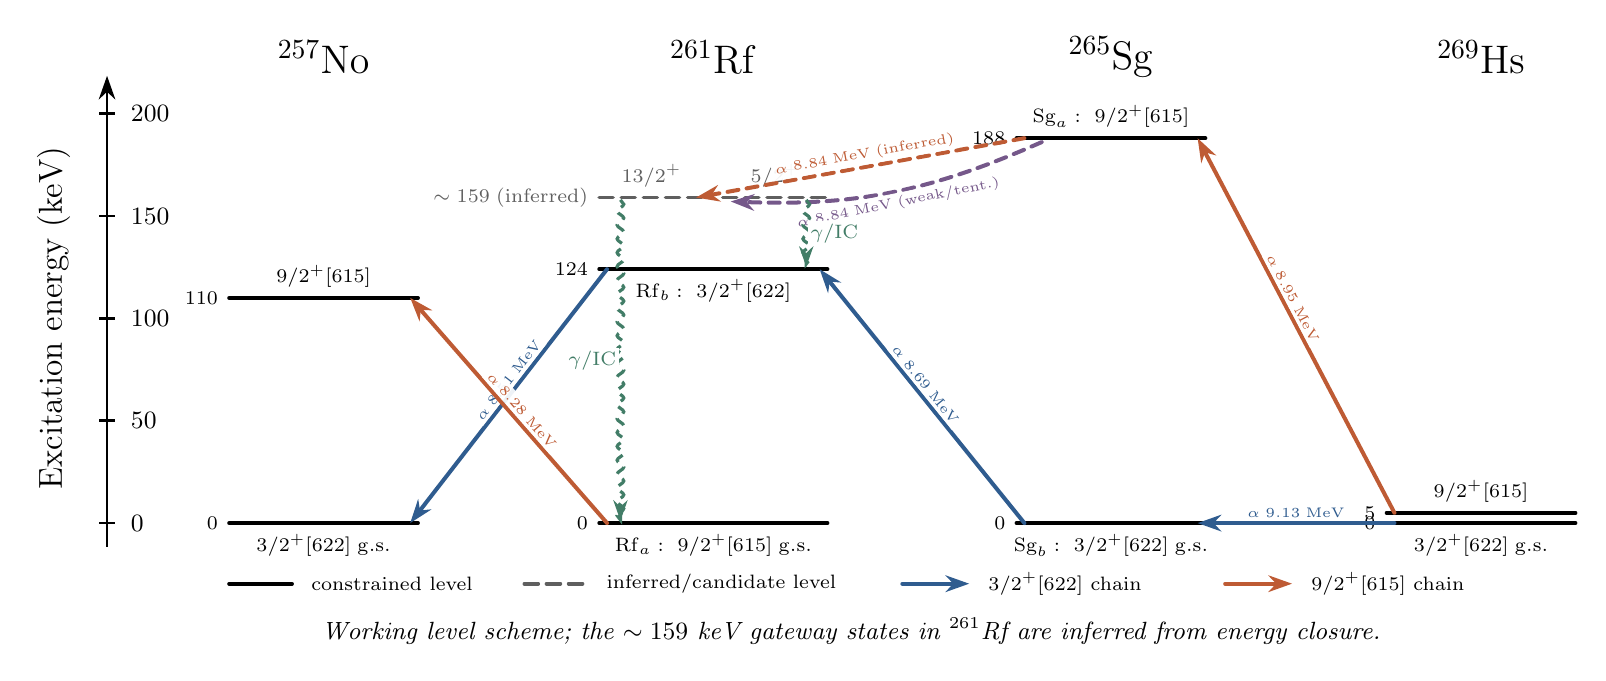
\begin{tikzpicture}[
    x=1cm,
    y=1cm,
    level/.style={
        line width=1.35pt,
        line cap=round
    },
    inferred level/.style={
        level,
        dash pattern=on 5pt off 3pt
    },
    transition/.style={
        -{Stealth[length=3.0mm,width=2.1mm]},
        line width=1.45pt,
        line cap=round
    },
    inferred transition/.style={
        transition,
        dash pattern=on 4pt off 3pt
    },
    gamma/.style={
        decorate,
        decoration={
            snake,
            amplitude=1.20pt,
            segment length=5.0pt
        },
        -{Stealth[length=2.6mm,width=1.8mm]},
        line width=1.15pt
    },
    inferred gamma/.style={
        gamma,
        dash pattern=on 3.5pt off 2.7pt
    },
    state/.style={
        font=\scriptsize,
        inner sep=1pt
    },
    energy/.style={
        font=\scriptsize,
        inner sep=1pt
    },
    nucleus/.style={
        font=\Large\bfseries
    },
    ticklabel/.style={
        font=\small
    },
    alphalabel/.style={
        font=\tiny,
        align=center,
        fill=white,
        fill opacity=0.92,
        text opacity=1,
        inner sep=1.2pt
    },
    note/.style={
        font=\scriptsize,
        align=center
    }
]

% ============================================================
% Muted scientific colors, following energylevelTentative.tex
% ============================================================

\definecolor{lowspinblue}{RGB}{47,92,143}
\definecolor{highspinorange}{RGB}{190,91,52}
\definecolor{alternativepurple}{RGB}{117,88,138}
\definecolor{gammagreen}{RGB}{66,125,103}
\definecolor{tentativegray}{RGB}{95,95,95}

% ============================================================
% Common excitation-energy scale
% ============================================================

\def\yZero{1.55}
\def\eScale{0.026}

\pgfmathsetmacro{\yFive}{\yZero + 5*\eScale}
\pgfmathsetmacro{\yOneTen}{\yZero + 110*\eScale}
\pgfmathsetmacro{\yOneTwoFour}{\yZero + 124*\eScale}
\pgfmathsetmacro{\yOneFiveNine}{\yZero + 159*\eScale}
\pgfmathsetmacro{\yOneEightEight}{\yZero + 188*\eScale}

\pgfmathsetmacro{\yFifty}{\yZero + 50*\eScale}
\pgfmathsetmacro{\yOneHundred}{\yZero + 100*\eScale}
\pgfmathsetmacro{\yOneFifty}{\yZero + 150*\eScale}
\pgfmathsetmacro{\yTwoHundred}{\yZero + 200*\eScale}

% Decay direction is from right to left.
\def\xAxis{0.00}

\def\xNoL{1.55}
\def\xNoR{3.95}

\def\xRfL{6.25}
\def\xRfR{9.15}

\def\xSgL{11.55}
\def\xSgR{13.95}

\def\xHsL{16.25}
\def\xHsR{18.65}

% ============================================================
% Excitation-energy axis
% ============================================================

\draw[line width=1.05pt]
    (\xAxis,1.25)
    --
    (\xAxis,{\yTwoHundred+0.15});

\draw[-{Stealth[length=3.0mm,width=2.1mm]},line width=1.05pt]
    (\xAxis,{\yTwoHundred+0.15})
    --
    (\xAxis,{\yTwoHundred+0.48});

\foreach \yy/\lab in {
    \yZero/0,
    \yFifty/50,
    \yOneHundred/100,
    \yOneFifty/150,
    \yTwoHundred/200
}{
    \draw[line width=1.0pt]
        (\xAxis-0.10,\yy)
        --
        (\xAxis+0.10,\yy);
    \node[ticklabel,anchor=west]
        at (\xAxis+0.18,\yy)
        {\lab};
}

\node[font=\large,rotate=90]
    at (\xAxis-0.68,{(\yZero+\yTwoHundred)/2})
    {Excitation energy (keV)};

% ============================================================
% Nucleus labels
% ============================================================

\node[nucleus] at ({(\xNoL+\xNoR)/2},{\yTwoHundred+0.72})
    {$^{257}\mathrm{No}$};
\node[nucleus] at ({(\xRfL+\xRfR)/2},{\yTwoHundred+0.72})
    {$^{261}\mathrm{Rf}$};
\node[nucleus] at ({(\xSgL+\xSgR)/2},{\yTwoHundred+0.72})
    {$^{265}\mathrm{Sg}$};
\node[nucleus] at ({(\xHsL+\xHsR)/2},{\yTwoHundred+0.72})
    {$^{269}\mathrm{Hs}$};

% ============================================================
% 257No levels
% ============================================================

\draw[level] (\xNoL,\yZero) -- (\xNoR,\yZero);
\node[state,anchor=north]
    at ({(\xNoL+\xNoR)/2},\yZero-0.10)
    {$3/2^{+}[622]\;\mathrm{g.s.}$};
\node[energy,anchor=east] at (\xNoL-0.10,\yZero) {$0$};

\draw[level] (\xNoL,\yOneTen) -- (\xNoR,\yOneTen);
\node[state,anchor=south]
    at ({(\xNoL+\xNoR)/2},\yOneTen+0.09)
    {$9/2^{+}[615]$};
\node[energy,anchor=east] at (\xNoL-0.10,\yOneTen) {$110$};

% ============================================================
% 261Rf levels and inferred gateway states
% ============================================================

\draw[level] (\xRfL,\yZero) -- (\xRfR,\yZero);
\node[state,anchor=north]
    at ({(\xRfL+\xRfR)/2},\yZero-0.10)
    {$\mathrm{Rf}_{a}:\ 9/2^{+}[615]\;\mathrm{g.s.}$};
\node[energy,anchor=east] at (\xRfL-0.10,\yZero) {$0$};

\draw[level] (\xRfL,\yOneTwoFour) -- (\xRfR,\yOneTwoFour);
\node[state,anchor=north]
    at ({(\xRfL+\xRfR)/2},\yOneTwoFour-0.09)
    {$\mathrm{Rf}_{b}:\ 3/2^{+}[622]$};
\node[energy,anchor=east] at (\xRfL-0.10,\yOneTwoFour) {$124$};

% The two near-degenerate candidates are split horizontally for clarity.
\draw[inferred level,tentativegray]
    (\xRfL,\yOneFiveNine) -- ({(\xRfL+\xRfR)/2-0.12},\yOneFiveNine);
\node[state,anchor=south,tentativegray]
    at ({(3*\xRfL+\xRfR)/4-0.06},\yOneFiveNine+0.09)
    {$13/2^{+}$};

\draw[inferred level,tentativegray]
    ({(\xRfL+\xRfR)/2+0.12},\yOneFiveNine) -- (\xRfR,\yOneFiveNine);
\node[state,anchor=south,tentativegray]
    at ({(\xRfL+3*\xRfR)/4+0.06},\yOneFiveNine+0.09)
    {$5/2^{+}$};
\node[energy,anchor=east,tentativegray]
    at (\xRfL-0.10,\yOneFiveNine) {$\sim159\;\mathrm{(inferred)}$};

% ============================================================
% 265Sg levels
% ============================================================

\draw[level] (\xSgL,\yZero) -- (\xSgR,\yZero);
\node[state,anchor=north]
    at ({(\xSgL+\xSgR)/2},\yZero-0.10)
    {$\mathrm{Sg}_{b}:\ 3/2^{+}[622]\;\mathrm{g.s.}$};
\node[energy,anchor=east] at (\xSgL-0.10,\yZero) {$0$};

\draw[level] (\xSgL,\yOneEightEight) -- (\xSgR,\yOneEightEight);
\node[state,anchor=south]
    at ({(\xSgL+\xSgR)/2},\yOneEightEight+0.09)
    {$\mathrm{Sg}_{a}:\ 9/2^{+}[615]$};
\node[energy,anchor=east] at (\xSgL-0.10,\yOneEightEight) {$188$};

% ============================================================
% 269Hs levels
% ============================================================

\draw[level] (\xHsL,\yZero) -- (\xHsR,\yZero);
\node[state,anchor=north]
    at ({(\xHsL+\xHsR)/2},\yZero-0.10)
    {$3/2^{+}[622]\;\mathrm{g.s.}$};
\node[energy,anchor=east] at (\xHsL-0.10,\yZero) {$0$};

\draw[level] (\xHsL,\yFive) -- (\xHsR,\yFive);
\node[state,anchor=south]
    at ({(\xHsL+\xHsR)/2},\yFive+0.09)
    {$9/2^{+}[615]$};
\node[energy,anchor=east] at (\xHsL-0.10,\yFive) {$5$};

% ============================================================
% Alpha-decay branches, directed from right to left
% ============================================================

% Low-spin 3/2+[622] chain.
\draw[transition,lowspinblue]
    (\xHsL+0.10,\yZero)
    -- node[alphalabel,above] {\alphaval{9.13}}
    (\xSgR-0.10,\yZero);

\draw[transition,lowspinblue]
    (\xSgL+0.10,\yZero)
    -- node[alphalabel,sloped,above,pos=0.52] {\alphaval{8.69}}
    (\xRfR-0.10,\yOneTwoFour);

\draw[transition,lowspinblue]
    (\xRfL+0.10,\yOneTwoFour)
    -- node[alphalabel,sloped,above,pos=0.46] {\alphaval{8.51}}
    (\xNoR-0.10,\yZero);

% High-spin 9/2+[615] chain.
\draw[transition,highspinorange]
    (\xHsL+0.10,\yFive)
    -- node[alphalabel,sloped,above,pos=0.56] {\alphaval{8.95}}
    (\xSgR-0.10,\yOneEightEight);

\draw[inferred transition,highspinorange]
    (\xSgL+0.10,\yOneEightEight)
    -- node[alphalabel,sloped,above,pos=0.48]
        {\alphaval{8.84}\;(inferred)}
    ({(\xRfL+\xRfR)/2-0.22},\yOneFiveNine);

\draw[transition,highspinorange]
    (\xRfL+0.10,\yZero)
    -- node[alphalabel,sloped,above,pos=0.47] {\alphaval{8.28}}
    (\xNoR-0.10,\yOneTen);

% Weak alternative feeding of the near-degenerate 5/2+ candidate.
\draw[inferred transition,alternativepurple]
    (\xSgL+0.32,\yOneEightEight-0.05)
    to[bend left=13]
    node[alphalabel,sloped,below,pos=0.48]
        {\alphaval{8.84}\;(weak/tent.)}
    ({(\xRfL+\xRfR)/2+0.22},\yOneFiveNine-0.05);

% ============================================================
% In-band gamma / internal-conversion de-excitation in 261Rf
% ============================================================

\draw[inferred gamma,gammagreen]
    (\xRfL+0.27,\yOneFiveNine-0.03)
    -- node[state,fill=white,inner sep=1pt,left] {$\gamma$/IC}
    (\xRfL+0.27,\yZero+0.03);

\draw[inferred gamma,gammagreen]
    (\xRfR-0.27,\yOneFiveNine-0.03)
    -- node[state,fill=white,inner sep=1pt,right] {$\gamma$/IC}
    (\xRfR-0.27,\yOneTwoFour+0.03);

% ============================================================
% Legend and schematic qualification
% ============================================================

\draw[level] (1.55,0.78) -- (2.35,0.78);
\node[note,anchor=west] at (2.47,0.78) {constrained level};

\draw[inferred level,tentativegray] (5.30,0.78) -- (6.10,0.78);
\node[note,anchor=west] at (6.22,0.78) {inferred/candidate level};

\draw[transition,lowspinblue] (10.10,0.78) -- (10.95,0.78);
\node[note,anchor=west] at (11.07,0.78) {$3/2^{+}[622]$ chain};

\draw[transition,highspinorange] (14.20,0.78) -- (15.05,0.78);
\node[note,anchor=west] at (15.17,0.78) {$9/2^{+}[615]$ chain};

\node[note,font=\small\itshape]
    at (9.45,0.18)
    {Working level scheme; the $\sim159$ keV gateway states in $^{261}$Rf are inferred from energy closure.};

\end{tikzpicture}

\end{document}
